\chapter{Revisão Bibliográfica}
\label{cap:revisao}

\section{A reação de transesterificação}

A transesterificação de um triglicerídeo com um álcool de cadeia curta produz
ésteres alquílicos de ácidos graxos e glicerol. Empregando-se metanol, a reação
global é escrita como

\begin{equation}
\mathrm{TG} + 3\,\mathrm{MeOH} \rightleftharpoons 3\,\mathrm{FAME} + \mathrm{GL}
\label{eq:global}
\end{equation}

\noindent
em que TG designa o triglicerídeo, FAME o éster metílico e GL o glicerol. A
estequiometria global, contudo, esconde o que de fato ocorre no meio reacional.
A conversão se dá por três etapas consecutivas e reversíveis, nas quais o
triglicerídeo é sucessivamente convertido a diglicerídeo, monoglicerídeo e
glicerol, liberando uma molécula de éster a cada passagem
\parencite{Noureddini1997}:

\begin{align}
\mathrm{TG}  + \mathrm{MeOH} &\rightleftharpoons \mathrm{DG} + \mathrm{FAME} \label{eq:etapa1}\\
\mathrm{DG}  + \mathrm{MeOH} &\rightleftharpoons \mathrm{MG} + \mathrm{FAME} \label{eq:etapa2}\\
\mathrm{MG}  + \mathrm{MeOH} &\rightleftharpoons \mathrm{GL} + \mathrm{FAME} \label{eq:etapa3}
\end{align}

O caráter reversível das três etapas impõe o emprego de excesso de álcool para
deslocar o equilíbrio na direção dos produtos. Razões molares entre
\num{6}:\num{1} e \num{12}:\num{1} de álcool para óleo são as mais comuns na
prática, contra o valor estequiométrico de \num{3}:\num{1}
\parencite{Freedman1986}. O excesso cumpre ainda uma segunda função, menos evidente:
ao manter a concentração de metanol praticamente constante ao longo da reação,
permite que a cinética seja tratada como de pseudo-primeira ordem no
triglicerídeo, simplificação de que este trabalho faz uso no
Capítulo~\ref{cap:modelagem}.

O excesso não é, entretanto, gratuito. Como observam \textcite{Allain2016}, o
álcool não convertido precisa ser recuperado a jusante do reator, e essa
separação responde por parcela apreciável do consumo energético do processo.
Em catálise heterogênea o excesso tende a ser ainda maior, justamente porque a
reação passa a ser limitada também pela difusão até o catalisador. Há portanto
um compromisso entre conversão por passe e custo de separação, que o projeto do
reator pode deslocar.

A escolha do modelo cinético empregado para descrever essa sequência não é
arbitrária, e \textcite{Ezzati2021} a sistematizaram em bases teóricas. Partindo
do mecanismo de três etapas, os autores derivaram uma equação de taxa geral,
válida ao longo de todo o tempo de reação, e mostraram a quais condições cada
modelo simplificado corresponde: a equação geral reduz-se ao modelo de segunda
ordem nos tempos iniciais de reação, e ao modelo de pseudo-primeira ordem nos
tempos iniciais com álcool em alta concentração. A conclusão que interessa
diretamente a este trabalho é a restrição: ao contrário do que a prática
corrente sugere, os modelos de pseudo-primeira e de segunda ordem são acurados
apenas nos tempos iniciais de reação, e não ao longo de toda ela.

Essa restrição é satisfeita no sistema aqui estudado, e por uma razão que
decorre do próprio resultado obtido. Como se mostra no
Capítulo~\ref{cap:resultados}, a conversão por passe no canal monolítico é de
\SI{1.4}{\percent}, de modo que o fluido percorre o reator permanecendo no
regime de tempos iniciais a que a aproximação de pseudo-primeira ordem se
aplica. A hipótese adotada na Seção~\ref{sec:bc} apoia-se nessa coincidência, e
deixaria de valer caso configurações de conversão elevada viessem a ser
simuladas.

Entre os fatores que governam o rendimento da reação, \textcite{Freedman1986}
identificaram a razão molar álcool/óleo, a temperatura, o teor de catalisador e
a presença de água e de ácidos graxos livres na matéria-prima. A temperatura de
operação é limitada superiormente pelo ponto de ebulição do metanol, de
\SI{64.7}{\celsius} à pressão atmosférica, de modo que a maior parte dos
trabalhos opera próximo a \SI{60}{\celsius} em sistema aberto, ou em pressões
moderadas quando se deseja ultrapassar esse limite.

\section{Limitações da rota homogênea}

A catálise alcalina homogênea, conduzida com hidróxido ou metóxido de sódio ou
potássio dissolvidos no metanol, continua a ser a rota predominante na indústria
por razões de desempenho. As velocidades de reação são elevadas, e conversões
superiores a \SI{95}{\percent} são alcançadas em menos de uma hora a
\SI{60}{\celsius}.

As dificuldades aparecem a jusante do reator. O catalisador permanece dissolvido
nos produtos e precisa ser neutralizado com ácido, operação que consome insumo e
gera uma corrente salina. A glicerina obtida carrega sais e metanol residual, o
que reduz seu valor comercial e exige purificação adicional. A separação das
fases demanda lavagens sucessivas com água, cuja corrente de saída retorna ao
processo como efluente a ser tratado.

Matérias-primas de menor custo agravam o quadro. Óleos residuais e gorduras
animais contêm ácidos graxos livres em teores que podem superar
\SI{5}{\percent}, e esses ácidos consomem o catalisador básico na formação de
sabões. Além de reduzir a quantidade de catalisador disponível para a reação
pretendida, os sabões formados estabilizam emulsões entre as fases éster e
glicerol, dificultando a separação e reduzindo o rendimento efetivo do processo.

\pendente{acrescentar dados quantitativos de consumo de insumos e geração de
efluentes, que as referências consultadas até aqui não trazem de forma
consolidada}

\subsection{A mistura bifásica e a limitação por transferência interfacial}
\label{sec:bifasico}

Há uma dificuldade anterior a todas as mencionadas, e que independe da natureza
do catalisador. Óleo vegetal e metanol têm polaridades muito distintas e
apresentam lacuna de miscibilidade: a mistura inicial de reagentes não é uma
solução, e sim um sistema líquido-líquido de duas fases, uma rica em óleo e
outra rica em álcool \cite{Muller2019}.

A consequência é que a taxa global passa a depender da transferência de massa
através da interface entre as fases, que é lenta em comparação com a reação
química. \textcite{Muller2019} observa que a etapa inicial da reação é
caracterizada por limitações difusionais severas, decorrentes justamente dessa
solubilidade mútua reduzida, e que o aumento da área interfacial por meios
mecânicos --- agitação, misturadores estáticos, sonicação, microrreatores ---
constitui a resposta habitual ao problema.

A situação se altera ao longo da conversão. Os ésteres formados atuam como
cossolvente entre as duas fases, e \textcite{Muller2019} registra que a mistura
se torna homogênea quando a reação atinge algo entre
\SIrange{15}{20}{\percent} de conversão, a partir do que a necessidade de mistura
intensiva diminui. A conversões ainda mais altas, o éster se separa da
glicerina, e o sistema volta a ser bifásico por outra razão.

Essa transição tem implicação direta sobre o presente trabalho, e é retomada na
Seção~\ref{sec:limitacoes}.

Registre-se, por fim, que a configuração de reator responde a essas
dificuldades de formas distintas. \textcite{Muller2019} contrasta a operação em
batelada, flexível quanto à matéria-prima mas de baixa produtividade e com
variação de qualidade entre bateladas, com a operação contínua, que oferece
qualidade mais constante e menor custo operacional por unidade de produto ao
preço de maior investimento e de controle de processo mais elaborado. Entre os
reatores contínuos, aponta os de leito fixo tubular como introduzidos
precisamente para superar as limitações intrínsecas de conversão dos reatores
com retromistura.

\section{Catálise heterogênea com óxido de cálcio}
\label{sec:cao}

A imobilização do catalisador em uma fase sólida elimina, de uma só vez, a
neutralização, a contaminação da glicerina e boa parte das lavagens. O
catalisador pode ser recuperado por filtração ou, no caso de um reator de leito
fixo ou de parede catalítica, simplesmente permanece no equipamento.

Entre os sólidos básicos investigados para a reação, o óxido de cálcio reúne
características que explicam sua posição de destaque na literatura: basicidade
suficiente para catalisar a reação em temperaturas brandas, custo baixo,
toxicidade reduzida e possibilidade de obtenção a partir de resíduos
carbonáticos, como cascas de ovo, conchas e carapaças, por calcinação. A
atividade do CaO está associada aos sítios básicos de Lewis formados pelos
pares O$^{2-}$ na superfície, que abstraem o próton do metanol e geram o íon
metóxido, espécie que efetivamente ataca o carbono carbonílico do
triglicerídeo.

Duas limitações do CaO são recorrentemente apontadas. A primeira é a lixiviação
de cálcio para o meio reacional, que introduz uma contribuição homogênea à
conversão observada e reduz a vida útil do catalisador ao longo de ciclos
sucessivos. A segunda é a sensibilidade à água e ao dióxido de carbono
atmosféricos, que convertem a superfície a hidróxido e a carbonato,
desativando-a; por essa razão o catalisador é normalmente calcinado
imediatamente antes do uso.

A lixiviação foi quantificada por \textcite{Melo2023} em condições próximas das
aqui simuladas. Medindo o teor de Ca$^{2+}$ no biodiesel produzido, o autor
obteve \SI{585(375)}{\milli\gram\per\kilogram} para o CaO não suportado e
\SI{40(26)}{\milli\gram\per\kilogram} para o CaO depositado em biochar de bagaço
de cana. Os dois valores excedem o limite de \num{5} ppm fixado pela
ANP n\textsuperscript{o} 45/2014, pela ASTM D6751 e pela EN 14214, mas o suporte
reduz o arraste de cálcio por um fator próximo de quinze. O autor atribui essa
retenção aos grupos funcionais oxigenados do biochar ativado, que ancorariam o
cálcio à matriz carbonácea, possivelmente por ligações O--Ca--O.

A desativação ao longo de ciclos sucessivos tem origem distinta da lixiviação, e
igualmente relevante para a operação contínua. \textcite{Melo2023} observou
queda acentuada de atividade entre ciclos, chegando a \SI{49.4}{\percent} de
conversão no segundo e a conversão nula no terceiro, a depender do procedimento
de lavagem empregado, e atribuiu o efeito ao acúmulo de glicerídeos e glicerol
aderidos à superfície do catalisador, confirmado por microscopia eletrônica.
Nenhum dos cinco procedimentos de lavagem ensaiados restabeleceu plenamente a
atividade.

Esses dois mecanismos, arraste de cálcio e bloqueio da superfície, não são
tratados pelo modelo desenvolvido neste trabalho, que é isotérmico e de estado
quase-estacionário. Condicionam, porém, a viabilidade prática da configuração e
definem o horizonte de operação que o reator pode sustentar antes de exigir
regeneração.

Duas dissertações recentes do mesmo programa de pós-graduação forneceram os
parâmetros empregados na presente modelagem.
\textcite{Melo2023} estudou a metanólise de óleo de soja sobre CaO suportado
em biochar a \SI{65}{\celsius}, obtendo a constante cinética por massa de
catalisador adotada no Capítulo~\ref{cap:modelagem}. \textcite{Fonseca2026}
investigou a rota etílica com CaO e CaO/Al$_2$O$_3$ a \SI{70}{\celsius} e razão
molar óleo:etanol de \num{1}:\num{9}, reportando difusividades efetivas no
interior do catalisador na faixa de \SIrange{3e-13}{4.4e-12}{\meter\squared\per\second},
valores que sustentam a estimativa do fator de efetividade apresentada na
Seção~\ref{sec:thiele}.

\section{Reatores monolíticos de parede catalítica}

Um monólito catalítico consiste em um bloco cerâmico ou metálico atravessado por
um grande número de canais paralelos de seção reta pequena, cujas paredes são
recobertas por uma camada fina de material catalítico, denominada
\textit{washcoat}. A densidade de canais é expressa em células por polegada
quadrada, e valores entre \num{200} e \num{600}~cpsi são usuais.

A geometria oferece duas vantagens sobre o leito fixo convencional. A razão
entre área superficial e volume é consideravelmente maior, o que aumenta a área
disponível para reação por unidade de volume de reator. E, como o escoamento se
dá em canais retos e abertos, a perda de carga é muito inferior à de um leito de
partículas, o que reduz o custo de bombeamento e viabiliza vazões elevadas.

A simulação de um monólito completo é inviável e, felizmente, desnecessária. A
simetria do arranjo permite tratar um único canal como representativo do
conjunto, hipótese consagrada na modelagem de conversores catalíticos e
discutida em detalhe por \textcite{HayesKolaczkowski1997}. A condição que a
justifica é que a distribuição de vazão entre os canais seja razoavelmente
uniforme e que não haja gradientes térmicos relevantes na direção transversal ao
feixe. Em um reator isotérmico operando em regime laminar, como o deste
trabalho, ambas as condições são satisfeitas com folga.

A deposição do \textit{washcoat} é a etapa crítica da fabricação. A camada deve
ser espessa o suficiente para comportar massa útil de catalisador, mas fina o
bastante para que o reagente alcance os sítios ativos no interior do poro antes
de ser consumido na entrada deles. Esse compromisso é quantificado pelo módulo
de Thiele e discutido na Seção~\ref{sec:thiele}.

\subsection{Aplicação à produção de biodiesel}

A transposição da configuração monolítica para a transesterificação é recente e
ainda pouco explorada em comparação com suas aplicações consagradas em
tratamento de gases de exaustão. Dois trabalhos desenvolvidos na University of
Bath constituem a referência mais direta para o presente estudo.

\textcite{Asli2011} recobriu monólitos de cordierita de \SI{62}{\per\centi\meter\squared}
com prolinato de zinco e avaliou o desempenho tanto em reator batelada quanto
em escoamento contínuo. Em batelada, com razão molar metanol:óleo de colza de
\num{12}:\num{1} a \SI{195}{\celsius} e \SI{20}{\bar} por duas horas, obteve
conversões elevadas, mas observou perda progressiva de atividade. No reator
contínuo, com tubo de \SI{6.2}{\milli\meter} de diâmetro interno carregado com
segmentos de monólito recobertos e comprimentos empacotados de \SI{200}{\milli\meter} e
\SI{400}{\milli\meter}, as conversões se mantiveram altas por \SIrange{100}{200}{\minute},
mas a desativação persistiu. A causa foi identificada por medida direta: o zinco
lixiviava para o meio reacional ao longo do ensaio. O trabalho registra ainda
que o próprio suporte de cordierita apresentou atividade catalítica, o que
complica a atribuição da conversão observada ao recobrimento, e encerra com
ensaios exploratórios empregando SrO sobre o mesmo suporte.

\textcite{Firth2014} desenvolveu a linha em direção ao escoamento contínuo.
Após triagem que descartou óxido de lantânio modificado por lentidão
--- vinte e quatro horas para \SI{94}{\percent} de conversão ---, selecionou
óxido de estrôncio, que alcançou \SI{95}{\percent} do rendimento teórico em
cinco minutos. O recobrimento por impregnação de nitrato exigiu temperaturas
elevadas e formou aluminato de estrôncio, menos ativo, com carga entre
\SIrange{5.7}{6.2}{\percent} e atividade irregular; o recobrimento por
suspensão de hidróxido de estrôncio alcançou carga de \SI{24}{\percent} em
massa, mecanicamente estável e reprodutível em peças maiores.

Em reator de canal único, com \SI{6.2}{\milli\meter} de diâmetro interno e
\SI{400}{\milli\meter} de comprimento aquecido a \SI{195}{\celsius} e tempo de
residência próximo de \SI{30}{\minute}, obteve conversão de triglicerídeo de
\SI{65.4}{\percent} mantida ao longo de cem horas. Em sua condição mais ativa,
o sistema converteu integralmente o triglicerídeo em meia hora de residência,
tempo que o autor estima ser cerca de quatro vezes menor que o do processo
heterogêneo industrial em condições comparáveis. Registrou, por outro lado,
oscilações de atividade entre conversão completa e \SI{34.4}{\percent} ao longo
de trezentas horas, cuja causa não foi determinada, descartadas água na carga e
lixiviação do catalisador.

O reator de múltiplos canais, cinco tubos de \SI{22}{\milli\meter} de diâmetro
interno e \SI{550}{\milli\meter} em série, produziu o resultado que mais
interessa a este trabalho. A taxa de reação mostrou-se fortemente dependente da
vazão, e dessa dependência o autor infere que a reação permanecia limitada por
transferência de massa, mesmo depois de vencida a fase inicial de inibição por
triglicerídeo. Essa inibição inicial foi atribuída principalmente ao efeito da
viscosidade elevada nas condições de partida, e não à difusividade, uma vez que
a taxa não variou com a concentração de FAME na menor vazão ensaiada.

Três pontos desses trabalhos merecem ser retidos.

O primeiro é a origem da geometria adotada no Capítulo~\ref{cap:modelagem}. A
densidade de \SI{62}{\per\centi\meter\squared} empregada por
\textcite{Asli2011} equivale a \num{400} células por polegada quadrada, valor
usual em substratos comerciais de cordierita. A essa densidade corresponde um
passo de célula de \SI{1.27}{\milli\meter} e, descontada a espessura típica de
parede do substrato, uma abertura de canal próxima de \SI{1.1}{\milli\meter} ---
que é a altura adotada neste trabalho.

O segundo é a solubilidade mútua entre metanol e óleo, que condiciona a
hipótese de fase única adotada no Capítulo~\ref{cap:modelagem}.
\textcite{Firth2014} mediu quanto metanol se dissolve no óleo vegetal em função
da temperatura e obteve razão molar de \num{3}:\num{1} a \SI{65}{\celsius},
\num{6}:\num{1} a \SI{100}{\celsius} e \num{9}:\num{1} a \SI{120}{\celsius}.
Ou seja, à temperatura de operação aqui adotada, apenas o equivalente
estequiométrico se dissolve, e o excesso de álcool tende a constituir fase
separada. A consequência é discutida na Seção~\ref{sec:limitacoes}.

O terceiro é a desativação por lixiviação. O zinco lixiviado reportado por
\textcite{Asli2011} é o mesmo fenômeno descrito na Seção~\ref{sec:cao} para o
cálcio em catalisadores de CaO, e aparece ali em uma configuração monolítica,
isto é, exatamente na geometria aqui investigada. Trata-se de limitação de
estabilidade que o presente modelo não aborda, por ser isotérmico e de estado
quase-estacionário, mas que condiciona a viabilidade prática da configuração e
precisa ser enfrentada experimentalmente.

Convém, por fim, registrar o que distingue o presente trabalho dos anteriores.
Os estudos citados abordam o reator monolítico predominantemente pela via
experimental, medindo conversões em função das condições operacionais. A
contribuição pretendida aqui é de outra natureza: trata-se de resolver o campo
de concentração no interior do canal e extrair dele o regime de operação, de
modo a responder não apenas quanto se converte, mas qual resistência governa a
conversão e, por consequência, sobre qual variável de projeto atuar.

\section{Resistência interna: módulo de Thiele e fator de efetividade}
\label{sec:thiele}

Dentro da camada porosa, reação e difusão competem. Se a reação for lenta em
relação à difusão, o reagente penetra toda a espessura do \textit{washcoat} e
todo o catalisador depositado trabalha na concentração da superfície externa. Se
a reação for rápida, o reagente é consumido nas primeiras camadas e o interior
permanece ocioso.

Para uma camada plana de espessura $\delta_{wc}$ com reação de primeira ordem, a
razão entre as duas escalas de tempo é medida pelo módulo de Thiele,

\begin{equation}
\phi = \delta_{wc}\sqrt{\frac{k_v}{D_p}}
\label{eq:thiele}
\end{equation}

\noindent
em que $k_v$ é a constante cinética por volume de \textit{washcoat} e $D_p$ a
difusividade efetiva no interior do poro. A fração da atividade nominal
efetivamente aproveitada é dada pelo fator de efetividade,

\begin{equation}
\eta = \frac{\tanh \phi}{\phi}
\label{eq:efetividade}
\end{equation}

\noindent
que tende à unidade para $\phi \ll 1$ e decai como $1/\phi$ para $\phi \gg 1$.

A consequência prática dessa dependência merece ser explicitada, por ser
frequentemente mal interpretada. A massa de catalisador por área de parede
cresce linearmente com $\delta_{wc}$, ao passo que $\eta$ decai; o produto dos
dois, que é o que determina a taxa observada, não passa por máximo. Substituindo
$\eta$ na taxa por área,

\begin{equation}
r_{obs} = \eta\, k_v\, \delta_{wc}\, C = C \sqrt{k_v D_p}\, \tanh \phi
\label{eq:rsat}
\end{equation}

\noindent
verifica-se que a taxa cresce monotonicamente e satura em $C\sqrt{k_v D_p}$,
valor independente da espessura. A Figura~\ref{fig:thiele} ilustra os dois
comportamentos. O que se perde ao engrossar a camada além do joelho da curva não
é taxa, e sim material: o catalisador é depositado, ocupa volume e custa, mas não
contribui para a conversão.
\begin{figure}[htb]
\centering
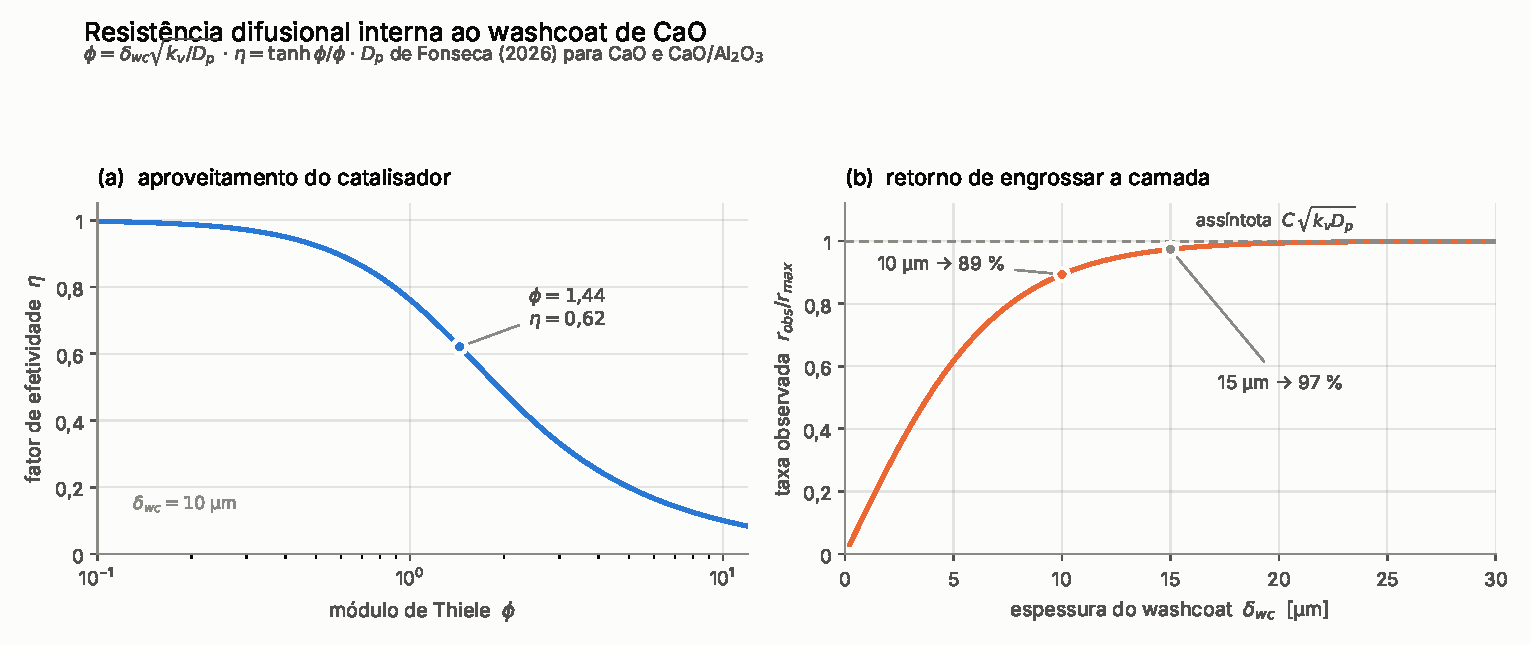
\includegraphics[width=\textwidth]{fig5_thiele_washcoat.pdf}
\caption{Resistência difusional interna ao \textit{washcoat}.
(a)~fator de efetividade em função do módulo de Thiele, com o ponto de operação
adotado neste trabalho; (b)~taxa observada em função da espessura da camada,
normalizada pela assíntota $C\sqrt{k_v D_p}$}
\label{fig:thiele}
\end{figure}

\section{Resistência externa: a camada-limite de concentração}
\label{sec:leveque}

Fora do \textit{washcoat}, o reagente precisa atravessar a camada de fluido que
se empobrece junto à parede. Em escoamento laminar plenamente desenvolvido, com
reação iniciando-se em $x = 0$, a espessura dessa camada é dada pela solução de
Lévêque,

\begin{equation}
\delta_c(x) = \left( \frac{9\,D\,x}{\gamma} \right)^{1/3},
\qquad \gamma = \frac{6\,\bar{u}}{H}
\label{eq:leveque}
\end{equation}

\noindent
em que $\gamma$ é a taxa de cisalhamento junto à parede e $H$ a altura do canal.
A dependência com $x^{1/3}$ é lenta, o que significa que a camada demora a
crescer e que o comprimento necessário para que ela preencha a seção pode ser
muito maior do que a intuição sugere.

Esse comprimento é o comprimento de entrada mássica, estimado por

\begin{equation}
L_e \approx 0{,}05\, D_h\, Re\, Sc
\label{eq:entrada}
\end{equation}

\noindent
com $Re = \rho\,\bar{u}\,D_h/\mu$ e $Sc = \mu/(\rho D)$. O produto $Re\,Sc$ é o
número de Péclet mássico, e é nele que reside a particularidade do sistema
estudado: enquanto o número de Reynolds é pequeno, da ordem de \num{0.2}, o
número de Schmidt de um óleo vegetal ultrapassa \num{1e5}, de modo que o produto
permanece elevado. O Capítulo~\ref{cap:resultados} mostra as consequências
disso para a geometria simulada.

\section{Número de Damköhler e regimes de operação}
\label{sec:damkohler}

A competição entre a reação na parede e o transporte até ela é medida pelo
número de Damköhler de parede, definido como a razão entre a taxa de reação
avaliada na concentração do seio do fluido e o fluxo máximo que o transporte
externo é capaz de sustentar,

\begin{equation}
Da = \frac{r_w(C_b)}{k_m\,C_b}
\label{eq:damkohler}
\end{equation}

\noindent
em que $k_m$ é o coeficiente de transferência de massa. Para reação de primeira
ordem na parede, o balanço em regime permanente entre o que o transporte entrega
e o que a reação consome conduz a uma relação direta entre $Da$ e as
concentrações medidas,

\begin{equation}
\frac{C_w}{C_b} = \frac{1}{1 + Da}
\qquad \Longleftrightarrow \qquad
Da = \frac{C_b}{C_w} - 1
\label{eq:cwcb}
\end{equation}

\noindent
expressão que será empregada no Capítulo~\ref{cap:resultados} para extrair $Da$
diretamente do campo simulado, sem a necessidade de estimar $k_m$ por correlação.

Três regimes são distinguidos. Quando $Da \ll 1$, a reação é lenta em comparação
com o transporte, a concentração junto à parede é praticamente igual à do seio
do fluido e o sistema opera sob controle cinético; nessa situação não há
gradiente apreciável a vencer, e aumentar a área de contato não altera o
desempenho. Quando $Da \gg 1$, a reação consome o reagente assim que ele chega,
a concentração na parede tende a zero e o desempenho passa a ser ditado
exclusivamente pelo transporte. Entre os dois extremos situa-se o regime misto,
no qual as duas resistências são comparáveis e ambas precisam ser consideradas
no projeto.

A classificação do sistema em um desses regimes é, do ponto de vista deste
trabalho, a questão central. É dela que depende a resposta sobre se a geometria
monolítica se justifica para a aplicação pretendida.

Convém registrar que o regime misto não constitui exceção nesta reação. Ao
estudarem a transesterificação de trioleína com metanol sobre ZnAl$_2$O$_4$ em
leito fixo, \textcite{Allain2016} concluíram que a difusão dos triglicerídeos e
a cinética da primeira etapa limitam conjuntamente a conversão global do
sistema. Trata-se de sistema distinto do aqui estudado, com outro catalisador,
outra forma física e outra faixa de temperatura, mas a coexistência das duas
resistências é a mesma situação que o Capítulo~\ref{cap:resultados} identifica
para o canal monolítico com CaO.

\section{Modelagem CFD de reatores de parede catalítica}

A simulação de um canal catalítico requer a solução simultânea das equações de
continuidade e de quantidade de movimento, que fornecem o campo de velocidade, e
das equações de transporte das espécies químicas, acopladas à cinética na
superfície. A reação heterogênea pode ser incorporada de duas formas.

A primeira consiste em discretizar o \textit{washcoat} como uma região porosa
adicional, com suas próprias equações de transporte e um termo fonte
volumétrico. A abordagem é rigorosa, mas impõe custo computacional elevado: a
camada tem espessura da ordem de dezenas de micrômetros, contra milímetros do
canal, e resolvê-la exige malha muito refinada em uma região de pouco interesse
direto.

A segunda trata a reação como condição de contorno de fluxo de espécies na
parede, incorporando a resistência interna por meio do fator de efetividade da
Equação~\eqref{eq:efetividade}. O custo é modesto e a perda de informação é
limitada ao perfil de concentração no interior do poro, que raramente é o objeto
de interesse. Foi esta a abordagem adotada no presente trabalho, e sua
implementação é descrita na Seção~\ref{sec:bc}.

A formulação do transporte multicomponente merece atenção. A lei de Fick, na
qual o fluxo difusivo de cada espécie é proporcional ao seu próprio gradiente,
é a opção padrão dos códigos comerciais e adequada à maior parte das aplicações.
Ela carrega, entretanto, uma restrição pouco discutida: a conservação da massa
total exige que a soma dos fluxos difusivos se anule, condição que só é
satisfeita quando todas as difusividades são iguais entre si. A formulação de
Maxwell-Stefan não tem essa limitação, por satisfazer a restrição de soma por
construção, mas exige difusividades binárias para todos os pares de espécies,
dado raramente disponível para sistemas contendo triglicerídeos. As implicações
dessa escolha para o presente trabalho são tratadas na
Seção~\ref{sec:difusividades}.

\subsection{Aplicações recentes a reatores de biodiesel}

A literatura de simulação aplicada à produção de biodiesel tem se concentrado em
duas frentes, ambas distintas do presente estudo.

A primeira compara configurações de reator quanto ao desempenho global.
\textcite{Omranpour2024} modelaram a transesterificação de óleo de canola com
metanol sobre ácido tungstofosfórico sólido, confrontando um reator de leito
fixo com um reator de membrana de leito empacotado. O modelo é bidimensional e
heterogêneo, resolvido numericamente. Nas melhores condições identificadas,
\SI{180}{\celsius}, razão molar de \num{15}:\num{1} e vazão de alimentação de
\SI{0.5}{\milli\liter\per\minute}, a conversão de \SI{99.94}{\percent} foi
atingida com \SI{86}{\centi\meter} de reator de membrana contra
\SI{2.75}{\meter} de leito fixo --- uma redução de comprimento por um fator
próximo de três para a mesma conversão. O consumo energético estimado para uma
planta de \SI{8000}{\tonne} por ano resultou em \SI{1313}{\kilo\watt} contra
\SI{1352}{\kilo\watt}, diferença bem menor que a de comprimento.

Esse resultado é instrutivo para o presente trabalho por tratar justamente da
relação entre comprimento de reator e conversão, que o
Capítulo~\ref{cap:resultados} identifica como a limitação dominante do canal
monolítico simulado.

A segunda frente trata de reatores de microcanal. \textcite{Laziz2020}
reportaram conversão de \SI{98.6}{\percent} em \SI{40}{\second} de reação à
temperatura ambiente, em microcanal de \SI{690}{\micro\meter} de diâmetro
alimentado por junção em T, empregando óleo de palma e hidróxido de potássio.
A simulação tridimensional com modelo de volume de fluido revelou uma estrutura
de recirculação toroidal no interior do pistão de metanol, à qual os autores
atribuem a intensificação da transferência de massa através da interface
líquido-líquido. \textcite{Subramaniam2024} revisaram o estado da arte dessas
tecnologias, destacando a razão área/volume elevada, a intensificação da mistura
por geometria de canal, micromisturadores e padrões de escoamento em pistão, e o
aquecimento por irradiação de micro-ondas como vias de intensificação.

A aproximação entre microcanais e monólitos merece comentário, por não ser
imediata. Ambas as configurações reduzem a distância que o reagente percorre até
onde a reação ocorre, mas o fazem em regimes distintos. No trabalho de
\textcite{Laziz2020} o catalisador é hidróxido de potássio dissolvido, isto é, a
catálise é homogênea, e a resistência a vencer é a transferência de massa
através da interface entre duas fases imiscíveis; o que se intensifica é a
mistura. No monólito de parede catalítica a fase é única e a reação é
heterogênea, de modo que a resistência a vencer é o transporte difusivo até uma
superfície sólida. As conclusões de uma literatura não se transferem
automaticamente à outra, e a comparação precisa ser feita pelos grupos
adimensionais, e não pela semelhança geométrica.
